\documentclass[11pt]{article}
\usepackage{listings}
\usepackage{tikz}
\usepackage{fontspec}
\setmainfont{Latin Modern Roman}
\usetikzlibrary{arrows,automata,shapes}
\tikzstyle{block} = [rectangle, draw, fill=blue!20, 
    text width=5em, text centered, rounded corners, minimum height=2em]
\tikzstyle{bt} = [rectangle, draw, fill=blue!20, 
    text width=1em, text centered, rounded corners, minimum height=2em]

\newtheorem{defn}{Definition}
\newtheorem{crit}{Criterion}
\newcommand{\true}{\mbox{\sf true}}
\newcommand{\false}{\mbox{\sf false}}

\newcommand{\handout}[5]{
  \noindent
  \begin{center}
  \framebox{
    \vbox{
      \hbox to 5.78in { {\bf Software Testing, Quality Assurance and Maintenance } \hfill #2 }
      \vspace{4mm}
      \hbox to 5.78in { {\Large \hfill #5  \hfill} }
      \vspace{2mm}
      \hbox to 5.78in { {\em #3 \hfill #4} }
    }
  }
  \end{center}
  \vspace*{4mm}
}

\newcommand{\lecture}[4]{\handout{#1}{#2}{#3}{#4}{Lecture #1}}
\topmargin 0pt
\advance \topmargin by -\headheight
\advance \topmargin by -\headsep
\textheight 8.9in
\oddsidemargin 0pt
\evensidemargin \oddsidemargin
\marginparwidth 0.5in
\textwidth 6.5in

\parindent 0in
\parskip 1.5ex
%\renewcommand{\baselinestretch}{1.25}

\usepackage[listings]{tcolorbox}
\newtcbinputlisting{\codelisting}[3][]{
    extrude left by=1em,
    extrude right by=2em,
    listing file={#3},
    fonttitle=\bfseries,
    listing options={basicstyle=\ttfamily\footnotesize,numbers=left,language=Java,#1},
    listing only,
    hbox,
}
\newenvironment{itemizep}{
 \begin{itemize}
  \setlength{\itemsep}{0pt}
  \setlength{\parsep}{3pt}
  \setlength{\topsep}{3pt}
  \setlength{\partopsep}{0pt}
  \setlength{\leftmargin}{1.5em}
  \setlength{\labelwidth}{1em}
  \setlength{\labelsep}{0.5em} }
 {\end{itemize}}

 \newenvironment{enumeratep}{
 \begin{enumerate}
  \setlength{\itemsep}{0pt}
  \setlength{\parsep}{3pt}
  \setlength{\topsep}{3pt}
  \setlength{\partopsep}{0pt}
  \setlength{\leftmargin}{1.5em}
  \setlength{\labelwidth}{1em}
  \setlength{\labelsep}{0.5em} }
 {\end{enumerate}}

\begin{document}

\lecture{25 --- March 8, 2017}{Winter 2017}{Patrick Lam}{version 1}

We will see techniques for improving test design today, particularly
with respect to verifying results.

Reference: Gerard Meszaros. \emph{xUnit Test Patterns: Refactoring Test Code}. [Highly recommended. Available in the DC library.]

\paragraph{Goal.} Well-designed tests are \emph{self-checking}.
That means that if the test runs with no errors and no failures (and
hence produces a green bar in your IDE), we know that the test was
successful.

\begin{center}
    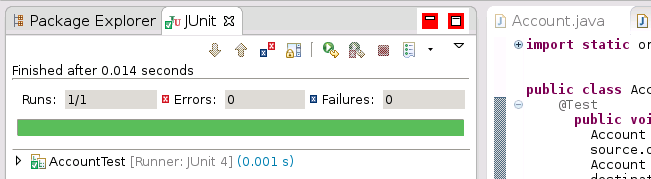
\includegraphics[width=.6\textwidth]{L25/pass}
\end{center}
  
Writing self-checking tests means that the tests automatically report
the status of the code. This enables a ``keep the bar green'' coding
style. Implications: 1) you can worry less about introducing bugs (but
still take ordinary care); and 2) the tests help document your
system's specs.

\paragraph{How to write self-checking tests.}
One might think:
\begin{quote}
  ``Isn't it just calling asserts?''
\end{quote}

Sadly, no. That's not enough.

Two questions about actually deploying asserts:
\begin{itemizep}
\item Q: what for?\\
  A: check method call results
\item Q: where?\\
  A: usually after calling SUT (System Under Test)
\end{itemizep}

\newpage
\paragraph{Counter example.} Here's some example code.
\codelisting{}{L25/Counter.java}
We can test it with the following JUnit test.
\codelisting{}{L25/CounterTest.java}

What kind of test is this? Let's consider two kinds of
tests: state-based tests vs. behaviour-based tests.

\begin{itemizep}
\item {\bf State:} e.g. object field values.
    Verify by calling accessor methods.
  \item {\bf Behaviour:} which calls SUT makes.
    Verify by inserting observation points, monitoring interactions.
\end{itemizep}

Does Counter Test verify state or behaviour?

\paragraph{Flight example.} Here's more example code.
\codelisting{}{L25/flight.java}

\subsection*{Implementing State Verification}
We can verify state:
\codelisting{}{L25/flight_extended_state_spec.java}

Note that we are exercising the SUT, verifying state,
and checking return values.

In state-based tests, we inspect only outputs, and only call methods from SUT. We do not instrument the SUT. We do not check interactions.

You have two options for verifying state:
\begin{enumeratep}
\item procedural (bunch of asserts); or,
\item via expected objects (stay tuned).
\end{enumeratep}

Returning to the flight example:
\begin{itemizep}
\item We do check that the flight got removed.
\item We don't check that the removal got logged.
\item Hard to check state and observe logging.
\item Solution: Spy on SUT behaviour.
\end{itemizep}

\newpage
\subsection*{Implementing Procedural Behaviour Verification}
Or, we can implement behaviour verification. This is one
way to do so, behaviourally:
\codelisting{}{L25/flight_pbv.java}

As an alternative, we can use a mock object framework (e.g. JMock) to
define expected behaviour.

\paragraph{Idea.} Observe calls to the logger,
make sure right calls happen.

\subsection*{Assertions}
We build tests using assertions. 
In JUnit, there are three basic built-in choices:
\begin{enumeratep}
\item assertTrue(aBooleanExpression)
\item assertEquals(expected, actual)
\item assertEquals(expected, actual, tolerance)
\end{enumeratep}
(There are others too, but let's start with these.)

{\tt assertTrue} is more flexible, since you can
write anything with a boolean value. However, it can give
hard-to-diagnose error messages---you need try harder when using it
if you want good tests.

\paragraph{Using Assertions.}
Why use assertions? Assertions are good for:
\begin{itemizep}
\item checking all the things that should be true (more = better);
\item serving as documentation:
    when system in state $S_1$,
    and I do $X$,
    assert that the result should be $R$, and
    that system should be in $S_2$.
\item allowing failure diagnosis (include assertion messages!)
\end{itemizep}

There are alternatives to using assertions.
For instance, one can also do external result verification:
\begin{itemizep}
\item write output to files; and
\item use diff (or your own custom diff) to compare
  expected and actual output.
\end{itemizep}

The twist is that the expected result is then not visible when looking
at test's source code. (What's a good workaround?)

\paragraph{Verifying Behaviour.} The key is to observe actions
(calls) of the SUT. Some options for doing this:
\begin{itemizep}
\item procedural behaviour verification
  (the challenge in that case: recording and verifying behaviour); or
\item expected behaviour specification
  (capturing the outbound calls of the SUT).
\end{itemizep}

\section*{How to Improve Your Tests}
Next, we'll talk about some techniques for improving your test cases.
Some tests are just better designed than others, making them easier
to maintain and to understand. Applying these techniques will help.

\paragraph{Reducing Test Code Duplication.}
Copy-pasting is common when writing tests. This results in
duplicate code in test cases, which has some undesirable
side effects (bloat, unnecessary asserts). We'll talk about
some techniques to mitigate duplication:
\begin{itemizep}
\item Expected Objects
\item Custom Assertions
\item Verification Methods
\end{itemizep}

Let's start with an example. One might expect many test methods like
this one.
\codelisting{}{L25/testInvoice.java}

\paragraph{Using an Expected Object.} We can compare objects instead:
\codelisting{}{L25/testInvoice-equality.java}

What we need:
\begin{itemizep}
\item a way to create the Expected Object;
\item a suitable {\tt equals()} method.
\end{itemizep}

Here are some potential barriers: 
\begin{itemizep}
\item we might need a special {\tt equals()} method, \\
  e.g. to compare subset of fields; or,
\item we may only have an {\tt equals()} that checks identity; or,
\item we can't create the desired expected object.
\end{itemizep}

Some solutions:
\begin{itemizep}
\item we can create a custom assertion; or,
\item we can provide special {\tt equals()} on expected object.
\end{itemizep}

\paragraph{Custom Assertions Example.} Consider the
following code:
\codelisting{}{L25/testInvoice-custom-assertion.java}

Tips:
\begin{itemizep}
\item Pick a good, declarative name.
\item Create the custom assertion by refactoring, using usual techniques.
\end{itemizep}

\paragraph{Benefits of Custom Assertions.}
Writing custom assertions can help with your test design. They:
\begin{itemizep}
  \item hide irrelevant detail;
  \item label actions with a good name (names are super important); and
  \item are themselves testable;
\end{itemizep}

\paragraph{Variant: Outcome-describing Verification Method.}
Instead of using a custom assertion, you might use a verification
method, like this one:

\codelisting{}{L25/testInvoice-verification-method.java}

Note that the verification method also interacts with SUT, but
may have arbitrary parameters.

\paragraph{Going Further: Parameterized, Data-Driven Tests.}
While we're at it,
there might be entire tests 
that differ only in input data.

Concrete tests invoke parametrized tests.

\newpage
\section*{Other Best Practices for Tests}
Avoid logic in tests.

The root problem is that tests are pretty much untestable.
If you including ifs and loops in tests, you're asking for trouble.
How are you going to make sure they're right?

\paragraph{Conditionals.} For example,
\codelisting{}{L25/BadConditional.java}
Instead, do this:
\codelisting{}{L25/GoodConditional.java}
The guard keeps you out of trouble.

\paragraph{Loops.}
    Don't put loops directly in tests.
    Use a well-named, testable Test Utility Method instead.

\section*{Summary}
In this lecture, we saw practical techniques for writing tests.
This included techniques for result verification (using state
verification and behaviour verification), as well as techniques
for improving your tests by reducing duplication and by simplifying
your tests.
\end{document}
